\documentclass[]{report}
%[dvips]
\usepackage{graphicx}
\usepackage{tabularx}
\usepackage{subfigure}
\usepackage{afterpage}
\usepackage{amsmath,amssymb}            
\usepackage{rotating}  
\usepackage{fancyhdr}  
\usepackage[scriptsize]{caption} 
\usepackage{url}
\hyphenation{a-gen-tiz-za-zio-ne}


%\addtolength{\oddsidemargin}{-0.5 cm}
%\addtolength{\evensidemargin}{-0.8 cm}
%\addtolength{\textwidth}{2.3 cm}
%\addtolength{\topmargin}{-2.20 cm}
%\addtolength{\textheight}{4.45 cm}
\linespread{1.1}

\usepackage[english]{babel}
\usepackage[latin1]{inputenc}
\renewcommand{\captionfont}{\normalfont \sffamily \itshape \small}

\pagestyle{fancy}

\begin{document}

\pagenumbering{Roman}
\renewcommand{\headrulewidth}{0 pt} 
\thispagestyle{empty}
%\begin{titlepage}
\vspace*{-1.5cm} \bfseries{
\begin{center}
	
	\large
  		POLITECNICO DI MILANO\\
  	
  	\normalsize
  		Corso di Laurea \textbf{MAGISTRALE} in Ingegneria Informatica\\
  		Dipartimento di Elettronica e Informazione\\
  		
  	\begin{figure}[htbp]
   		\begin{center}
      		\includegraphics [width = 3.5 cm]{./pictures/logopm}
    	\end{center}
  	\end{figure}
  	
\end{center}

\vspace*{2 cm}
\begin{center}
  	
  	\vspace*{0.3 cm} \LARGE

	\textbf{}\\

	\vspace*{.75 true cm} \large
  
  		NECST Lab \\
  		Novel, Emerging Computing System Technologies Laboratory\\
  		
\end{center}

\vspace*{3.0 cm} \large

\begin{minipage}[b]{.45\linewidth}
	\begin{flushleft}
  		Relatore: \\
  		Correlatore: \\ 
	\end{flushleft}
\end{minipage}
\begin{minipage}[b]{.45\linewidth}
	\begin{flushright}
  		Tesi di Laurea di:\\ 
	\end{flushright}
\end{minipage}

\vspace*{0.5 cm}

\begin{center}
	Anno Accademico 2015-2016
\end{center} \clearpage

}


\normalfont \cleardoublepage
\vspace{17cm}
\thispagestyle{empty}
%\large
\begin{flushright}
\itshape{ To someone...}
\end{flushright}


\cleardoublepage
\newpage
\chapter*{Summary}

\addcontentsline{toc}{chapter}{Summary}

\chapter*{Thanks}

\addcontentsline{toc}{chapter}{Thanks}


\pagenumbering{arabic}
\normalfont
\renewcommand{\chaptermark}[1]{\markboth{\thechapter.\ #1}{}} 
\renewcommand{\sectionmark}[1]{\markright{\thesection.\ #1}}         
%\fancyhead[LE,RO]{\bfseries\thepage}    
\fancyhead[RE]{\bfseries\leftmark}    
\fancyhead[LO]{\bfseries\rightmark}     
\renewcommand{\headrulewidth}{0.3 pt} 
\chapter{Introduction}
\label{Introduction}
\thispagestyle{empty}



\chapter{Motivation}
\label{chapter2}
\thispagestyle{empty}

\section{Problem statement}
\paragraph{}
In order to avoid Anti-Virus (AV) detection and harden the process of reverse engineering usually malware hide their code employing different techniques. This process, called \textit{packing}, makes the static analysis of a binary almost completely useless.\\
A \textit{packer} is the tool that implements the previously described functions: it receives in input a binary, transforms and obfuscates its code/resources and then appends new codes that will \textit{unpack} the original one runtime once the program is executed.\\
The complexity of \textit{packers} can be very different: from those which write and execute directly the original code, to others that employ multiple unpacking routines and obfuscation techniques such as runtime repacking of previously unpacked code.\\ A comprehensive study and a taxonomy of these levels of complexity have been made in a previous work. 
This process has different consequences both in the AV detection and manual analysis of malicious binary:
\begin{itemize}
\item Usually AV employ different static analysis techniques in order to understand if a file is malicious or not, but packing a binary destroys any possibility to understand what the program will do on the system without executing it.
\item The process of reverse engineering a packed malware can be very time consuming and since lots of malware is pushed every day on internet there is the necessity of fast analysis and fast updating of AV software.
\end{itemize}
\paragraph{}
These problems inspired different works in building an automatic generic unpacker aimed to extract the original code from the packed one. Some of them are more oriented in detection of malicious packed program helping an AV software on end users PCs, others are instead proposed as tools for speed up the work of professional malware analysts.

In order to clarify better what a packer is and how it operates we will discuss in the next capther the main points of the previously mentioned research.

\subsection{Packer taxonomy}
\paragraph{}
As previously explained a packer can implements different obfuscation techniques in order to harden the analysis of a program. In this paragraph we are going to analyze the proposed taxonomy in order to better understand the goals of our work and its limitation against the current packing methods.

Before starting to present the techniques we need to define some terms that are essential in order to understand how a packer works: 
\begin{itemize}
\item \textit{Layer}: a layer is a set of contiguous memory addresses that are executed after being written. A layer can unpack another layer or the original program code.
\item \textit{Transition}: a transition is a control transfer from a layer to another layer, it can be a \textit{forward transition} if the execution is going from a previously unpacked layer to a newer layer, or a \textit{backward transition} if the execution is going from a newer layer to an older one. From this definition we can derive the concept of \textit{linear unpacking} in which all the transition are \textit{forward transition}, and {cyclic unpacking} in which there are some \textit{forward transition} and some \textit{backward transition}. 
\item \textit{Tailed/Interleaved}: We say that a packer is tailed if there is soon or later a transition from the unpacker code to the original program code and then the execution never returns to the unpacker code, contrary we say that the unpacking is \textit{interleaved} if the execution bounce between the unpacker code and the original program code. 
\end{itemize}

We are going to identify the complexity of a packer by using a scale from 1 to 6.

\subsubsection{Type 1}

The simplest form of packer is the one that runtime unpack the original binary using only one layer and then jumps to it with a tail jump. 

<figura>

This scheme is typical of packers like UPX,FSG,EXEpacker.

\subsubsection{Type 2}

The packer in this category are defined as \textit{multi-layer} and \textit{linear}. This means that they employ different layer and the transition between them is always from the older to the newer. Also this kind of packers are defined as \textit{tailed} since the last jump redirect the execution at the original program code.

\subsubsection{Type 3}

Type 3 packers are defined as \textit{multi-layer}, \textit{cyclic} and \textbf{tailed}. This means that they employ different layers and the transitions are both \textit{forward transition} and \textit{backward transition}. 

\subsubsection{Type 4}

These packers are \textit{multi-layer}, \textit{cyclic} and \textbf{interleaved}. This means that they use different layers with both forward and backward transitions, and during the execution of the original program the control is redirected in some way to the packer code.

\subsubsection{Type 5}

\section{State of the art}
\paragraph{}
Lots of different tools using different approaches and techniques have been proposed. 
The approaches for automatic unpacking can be very different:
\begin{itemize}
\item \textit{Static unpacking}: this can sound counterintuitive, but some works proposed to identify unpacking routines inside the binary and reconstruct an ad hoc unpacker for the binary starting from these routines. This approach has got numerous limitation but can lead to interesting result in some case as demonstrated by Caballero et al.
\item \textit{Hybrid unpacking}: this mixes some static heuristics with dynamic analysis.
\item \textit{Dynamic unpacking}: these techniques follow the idea to let the unpacker do its work and then try to extract runtime the unpacked code. 
\end{itemize}
\paragraph{}
Depending on the purpose of the tool there are different requirements that a generic unpacker must respect. If the aim is to help the AV on end users' PCs:
\begin{itemize}
\item Safety: try to recognize the malicious behaviour as fast as possible and block the execution. 
\item Performance: it should not slow down too much the execution of AV scans.
\end{itemize}
Note that in these cases, the scope is not to reconstruct a binary from a packed one, but rather to stop malicious behaviours when they manifest. \\
In this area have been done works such as OmniUnpack and JustIn.
\paragraph{}
On the other side if the aim is to help the analysis in a laboratory:
\begin{itemize}
\item Fidelity: the unpacked binary extracted by the tool should be equal to the one that would be unpacked normally. 
\item Generality: the unpacker can not be focused only against one packer but should unpack different of them with one generic algorithm.
\end{itemize}
In this case we do not care so much about safety because usually analysis is performed inside a controlled environment and the analysts want to observe the complete execution of malware. Also the performances are not a critical feature here because we are not constrained by user experience needs.\\
In this category have been developed tools like PolyUnpack, Ether, Eureka, Renovo, Lynx.
These tools merely collect dumps of the binary while unpacking and they don't reconstruct a fully runnable binary given a packed one.


\section{Goals and challenges}
\paragraph{}
Since our work is born as a component of a bigger malware analysis platform (Jackdaw), our tool is oriented to help malware analyst during the reversing process of a packed binary. 
Our approach aims not only to unpack the malware, but also to reconstruct a fully working unpacked binary. To do so, we not only have to identify the original entry point (OEP) and dump the code at that moment, but we have to find the IAT inside the process and reconstruct a correct import directory in the final PE file.\\
The first thing we have to deal with are the unpacking routines of the packers: every time the execution of the malware comes from a previously written memory area, then it could be a sign that the unpacking stage has finished or that a new unpacking layer has started.\\
We have also to deal with techniques of IAT obfuscation: some malwares can do this in order to make difficult to statically analyse them to understand what they are doing.


\chapter{Approach}
\label{chapter3}
\thispagestyle{empty}

\section{Dynamic Binary Instrumentation}
\paragraph{}
Dynamic Binary Instrumentation is a technique for analysing the behaviour of a binary application through the injection of instrumentation code. The instrumentation code can be developed in an high level programming language and is executed in the context of the analysed binary with a granularity up to the single assembly instruction. The injection of instrumentation code is achieved by implementing a set of callbacks provided by the \ac{DBI} framework. The most common and useful callbacks are:
\begin{itemize}
 \item Instruction callback: invoked for each instruction
 \item Image load callback: invoked each time an image (dll or Main image) is loaded into memory
 \item Thread start callback: invoked each time a thread is started
\end{itemize}
Besides the callbacks the \ac{DBI} framework allows to intercept and modify operative system \acp{API} and system calls and this is very useful to track some behaviours of the binary, like the allocation of dynamic memory areas.

\section{Approach overview}
\paragraph{}
Our tool exploits the functionalities provided by the Intel PIN \ac{DBI} framework to track the memory addresses which are written and then executed with an instruction level granularity.
More in details for each instruction the following steps are performed:
\begin{enumerate}
\item Instruction Filtering: ignore the effects of a particular set of instructions for performance reasons
\item Written addresses tracking: keep track of each memory address which is written in order to create a list of memory ranges of contiguous writes defined \textit{Write Intervals} 
\item \textit{\ac{WxorX}} instructions tracking: check if the currently executed instruction belongs to a \textit{Write Interval}. This is a typical behaviour in a packer that is executing the unpacked layer and for this reason we trigger a detailed analysis which consists of:
	\begin{enumerate}
	\item Dumping the main image of the \ac{PE} and a memory range on the heap depending on the address of the current instruction
	\item Reconstructing the \ac{IAT} and generating the correct Import Directory
	\item Applying some heuristics to evaluate if the current instruction is the \ac{OEP}
	\end{enumerate}
\end{enumerate}
The result of our tool is a set of memory dumps or reconstructed \acp{PE} depending on the result of the \ac{IAT} fixing phase and a report which includes the values of each heuristic for every dump. Based on these information we can choose the best dump, that is the one that has the greatest chance of work.

\section{Approach details}
\paragraph{}
In this section we are going to describe in details the steps introduced in the previous section.
\paragraph{}
During the development we have adapted our approach in order to increase speed and effectiveness of our tool. Following there is a detailed explanation of our improvements on the initial approach:
\begin{enumerate}
\item in the first step, we add the option of not to track writes of library instructions on the stack and in the \ac{TEB}
\item in the second step we filter instructions of known libraries before dumping
	\begin{enumerate}
	\item when trying to reconstruct the \ac{IAT} we added some code in order to deal with 			obfuscation techniques like \textit{\ac{IAT} Redirection} and \textit{Stolen \ac{API}}
	\item we implemented five heuristics:
		\begin{itemize}
		\item entropy: check if the value of the entropy is above a certain threshold
		\item long jump: check if the "distance" between the current EIP and the previous 			one is above a certain threshold
		\item jump outer section: check if the current EIP is a different section from the 		one of the previous EIP
		\item pushad popad: check is a \textit{pushad-popad} pattern has been found in the trace
		\item init function calls: check if the imports of the dump are functions commonly 			 used by the malware and not by the unpacking layers
		\end{itemize}
	\end{enumerate}
\end{enumerate} 
For the instructions that execute from the same write set we adopted the following approach: if the "distance" between the current EIP and the EIP of the previous instruction is above a given threshold then we do the same as if we were in the case 2, otherwise we jump to the next instruction.\\
Finally, we have noticed that dumping only the main executable in memory is not enough because some packers dump the final payload on the heap. In order to deal with it, we track heap allocations and writes inside an heap interval. If necessary, we dump these intervals too.

\subsection{Instructions filtering}
\paragraph{}
Since our tool works with an instruction level granularity, limiting our analysis to the relevant instruction of the program is a critical point. For this reason we have introduced some filters, based on the common behaviours showed by the packers, which make our tool ignore the effects of a set of instructions. More in detail two kind of instructions are not tracked by default:
\begin{itemize}
	\item Write instruction on the \ac{TEB} and on the Stack
	\item Instruction executed by known Windows Libraries
\end{itemize}
The write instructions on the stack are ignored because unpacking code on the stack is not common compared to unpacking it on the heap or inside the main image. Moreover many instructions write on the stack and keeping track of all the written addresses would downgrade the performances gaining little advantages against a very small set of packers.\\
The same considerations can be applied to the instructions which write on the \ac{TEB}, since most of these writes are related to the creation of instruction handlers and there is very little chance that a packer uses this addresses to unpack the encrypted payload.\\
The instructions executed by known Windows Libraries are never considered when checking if the current instruction address is contained inside a \textit{Write Interval} because this would mean that the packer writes the malicious payload in the address space of a know Windows Library. This behaviour has never been identified in the packer analysed; moreover, this could introduce some crashes if the application explicitly use one of the functions which have been overwritten.

\subsection{Track WxorX instructions}
\paragraph{}
All packers, in order to work correctly, have to present a common behaviour: they must write the original program in memory and then they must execute the written code. We have defined an instruction that is first written by the packer and then executed as a \textit{WxorX instruction}.
Our tool tracks each write operation made by the program and build a set of memory ranges which identify contiguously written memory addresses. A memory range is dentified by a starting address and an end address and it is managed in order to take into account the memory operation that overlaps it (The starting address and the end address are decreased or increased 
respectively when an overlapping writes is detected).

\begin{figure}[H]
 \makebox[\textwidth][c]{\includegraphics[width=1.0\textwidth]{./pictures/wxorx_tracking.jpg}}%
\caption{Memory range management}
\end{figure} 

The first time we detect that the instruction pointer is inside one of our memory ranges, all the analysis and dumping routines (explained in the next chapters) are triggered and the memory range is marked as \textit{broken}. It is easy to deduct that the definition of a broken memory range is : A memory range in which the execution has been redirected to. 

\subsection{Heuristics description}
\paragraph{}
Our tool makes a dump each time the \ac{WxorX} law is broken in a new \textit{Write Interval} or in an existing one if \textit{InterWriteSet} analysis is enabled. Consequently, at the end of the execution we may have a lot of dumps and check them manually can be very time-consuming. Heuristics help in automatically identify the dumps that are most likely to work and also provide a "best dump", the one with the greatest chance to be the contain the original unpacked code. All the heuristics are described in \cite{Practical_Malware_Analysis}.
\paragraph{}
Entropy can be considered as a measure of the disorder of a program. For example, random data have the highest possible entropy. Since encrypted data more closely resembles random data, entropy can be used in detecting if an executable has been compressed, encrypted or both. Usually compressed files have less entropy that the original files, because the purpose of compression is to reduce the dimension of the file preserving some patterns used to recover the information. Encryption, on the opposite, has the goal of making unreadable a file, that is ideally changed in a random stream of bits. For example:\\
FFFFFFFFFFFFFFFFFFFF --------\textgreater 20'F' (compressed)\\
FFFFFFFFFFFFFFFFFFFF --------\textgreater ;LAKSDFJA;WIEFEJ;AEJF (encrypted)\\
As a result, while decompressing a file, its entropy slightly increase; while decrypting a file, its entropy slightly decrease. Consequently, in order to identify that a decompression or a decryption stage is finished, we have to check the absolute value of the difference between the initial and the current entropy.
\paragraph{}
It is very uncommon that the unpacking stub is located just under or above the \ac{OEP}. Instead, once the original code is fully unpacked, there is a long jump from the unpacking stub to the \ac{OEP} of the unpacked code. Sometimes, this jump has the target address is in a completely different section from the start address. This technique is called \textit{tail jump} and may be a sign of the completion of an unpacking stage. 
\begin{figure}[!ht]
	\begin{center}
   		\includegraphics [width=\textwidth]{./pictures/Original Code And Unpacking Stub.jpg}
	\end{center}
	\caption{Different jumps from the unpacking stub to the original code}
	\label{Original Code And Unpacking Stub}
\end{figure}
In Figure \ref{Original Code And Unpacking Stub}, the cases (a) and (b) are extremely rare, while case (c) is the most common.\\
We base on these considerations the \textit{long jump} and \textit{jump outer section} heuristics.
\paragraph{}
Usually packers employ a technique called \textit{pushad-popad}. The \textit{pushad} function stores on the stack the values of all the registers and the \textit{popad} function restores them in the registers. After a \textit{pushad}, a packer can execute its unpacking routine and soon before the \textit{tail jump} it can restore all the registers with a \textit{popad}. In this way, the two instructions almost delimit the unpacking stub and help to identify the range of memory addresses in which the \ac{OEP} is located. As an example, a commercial packer like \textit{ASPack} employs this technique.
\paragraph{}
When a malware is packed, it usually exhibits very few or false imports. This is a technique of obfuscation used by some packers in order to hide the real behaviour of the malware. Of course, it is a job of the packer to fully reconstruct the \ac{IAT} in order to make the binary runnable.\\
The purpose of the \textit{init function calls} heuristic is to search in the \ac{IAT} for functions commonly used by the malware and not by the unpacking stub. For example, if a malware has to contact an Internet domain to download some malicious code, it will have in its imports some internet communication \acp{API} like \textit{connect} and \textit{send}. Since the unpacking stub does not need them to perform its job, when packed the binary will not have these \acp{API} in its \ac{IAT}, but the packer will take care of inserting them among the imports during the unpacking stage. In some extreme cases, the packed binary may have as imports only the \textit{GetProcAddress} and \textit{LoadLibrary} functions, because these two are used to dynamically load libraries and functions.\\
Consequently, once identified some "interesting" \acp{API} for the malware but not for the packer, we check how many of them a dump has among its imports. Usually, the more of them, the higher the probability of being the correct dump.
\paragraph{}
\subsection{Evaluation of \textit{InterWriteSet} analysis}
\paragraph{}
The initial approach was to dump the code and trigger the analysis of if once the \ac{WxorX} law was broken in a \textit{Write Interval} for the first time and then ignore all the subsequent instructions from the same \textit{Write Interval}. However, when analysing a binary packed with \textit{mpress}, we noticed the behaviour in Figure \ref{mpress behaviour} that forced us to slightly modify the initial approach.\\
\begin{figure}[!ht]
	\begin{center}
   		\includegraphics [width=\textwidth]{./pictures/InterWriteSet Analysis - mpress.jpg}
	\end{center}
	\caption{Mpress behaviour}
	\label{mpress behaviour}
\end{figure}
When \textit{mpress} enters for the first time the \textit{Write Interval} which contains the original code (a), it jumps in an area of memory that contains a small stub that reconstructs the \ac{IAT} and then jumps to the original code (b), that resides in the same \textit{Write Interval}. With the original approach we were able to dump the code in (a), but we ignored the jump in (b) and so we were unable to recreate a running \ac{PE}.\\
Consequently, we adapted our approach to deal with this behaviour: we consider jumps inside the same \textit{Write Interval} only if they are longer than a given threshold. If this is the case, we trigger the analysis as if it was the first time the \ac{WxorX} law is broken. However, this improvement may potentially generate too many dumps, making the analysis very slow and difficult. For this reason there is a maximum number of jumps that are considered inside the same \textit{Write Interval}.
\chapter{Implementation details}
\label{chapter4}
\thispagestyle{empty}

\section{System architecture}
\paragraph{}
Our tool is entirely based on PIN, a binary instrumentation framework developed by Intel. It lets us to have the instruction-level granularity useful to track memory writes on a finer grain. In this way we are able, for example, to see where a single assembly write instruction is going to write and consequently create the write sets.\\
We have integrated Scylla, an external open source program, to dump the code and reconstruct the \ac{IAT}. Moreover we have extended it in order to deal with \textit{\ac{IAT} Redirection} and \textit{Stolen \ac{API}} techniques.\\
Finally we use the IDA Pro disassembler and an IDAPython script in the \textit{Init function calls} heuristic. The script calls IDA which reads the imports of the dump and compare them to a list of functions commonly used by the malware and not by the packer (registry manipulation, internet communication).

\section{System details}
\paragraph{}
In this section we are going to explain in detail the implementation of the most important parts of our tool.

\subsection{WriteSet management}
\paragraph{}
We introduce the concept of \textit{WriteInterval} in order to group together contiguous writes to check if an instruction executes from a previously written memory area. All the \textit{WriteIntervals} are grouped together in a \textit{WritesSet}, a simple C++ vector.\\
\paragraph{}
A \textit{WriteInterval} is a C++ structure with the following fields:
\begin{itemize}
\item addr\_begin: start address in memory of the \textit{WriteInterval}
\item addr\_end: end address in memory of the \textit{WriteInterval}
\item entropy\_flag: flag used by the \textit{Entropy Heuristic}
\item long\_jmp\_flag: flag used by the \textit{Long Jump Heuristic}
\item jmp\_outer\_section\_flag: flag used by the \textit{Jump Outer Section Heuristic}
\item pushad\_popad\_flag: flag used by the \textit{Pushad Popad Heuristic}
\item broken\_falg: flag which indicates if the \ac{WxorX} law has already been broken in this \textit{WriteInterval}
\item detectedFunctions: flag used in conjunction with the \textit{Init Function Call Heuristic} 
\item cur\_number\_jmp: current jump number, used to properly name the result file (see Section \ref{Dumping module})
\item heap\_flag: flag that indicates if the write is on the heap
\end{itemize}
For more information about heuristic see Section \ref{Heuristics implementation}.
\paragraph{}
The following steps explain how \textit{WriteIntervals} are created and updated:
\begin{enumerate}
\item for each instruction we check if it is a write
\item if so, we insert a \textit{callback} function before it. A \textit{callback} is a feature of PIN: it allows to instrument the code by inserting some code that will be executed before or after the original instruction. In our case, we intercept the write instruction and before the execution we retrieve its \ac{EIP}, the address where it will write and the size of the memory that will be written. With these information we compute the start and end addresses of the write
\item Now we proceed to the construction or the update of the \textit{WriteInterval}. We have five cases:
	\begin{enumerate}
	\item the memory written by the instruction neither is contained nor overlaps with another \textit{WriteInterval}. In this case we create a new one and add it to the \textit{WritesSet} vector
	\item the start address of the write is before the start of a \textit{WriteInterval}, but the end address is inside it. In this case we update the \textit{WriteInterval} setting as start address the start of the write, but leaving unaltered the end address
	\item the same as case (b), but this time regarding the end address. Consequently, we only update the end of the \textit{WriteInterval} 
	\item the memory written by the instruction completely contains a \textit{WriteInterval}. In this case we update both the start and the end of the \textit{WriteInterval}
	\item the memory written by the instruction is completely contained by an existing \textit{WriteInterval}. In this case we do nothing
	\end{enumerate}
\end{enumerate}
We check each instruction, including writes, to see if it executes from one of the \textit{WriteIntervals}. If this is the case, then we proceed with our analysis; in the other case we execute the instruction and go to the next one. In both cases the \textit{Write Intervals} are preserved, the reason will be clear in Section \ref{Dumping module}.\\

\subsection{Hooks of functions and syscalls}
\label{Hooks of functions and syscalls}
\paragraph{}
In order to make our tool properly work we have to hook some functions and system calls. We do this by inserting \textit{callback} functions before or after the original instruction and more rarely by completely replacing the original routine. We always try to hook functions at the lowest possible level.
\paragraph{}
When dumping code, we need to include also the code on the heap, because some packers unpack code in that memory area. In order to do this, we have to track all the heap allocations and deallocations in order to create an \textit{heapzone} in our tool.\\
An \textit{heapzone} is an abstraction of a heap area and is implemented as a C++ structure with the following fields:
\begin{itemize}
\item begin address
\item end address
\item size of the \textit{heapzone}
\end{itemize}
In order to manage the \textit{heapzones} we have to hook the following functions:
\begin{itemize}
\item \textit{RtlAllocateHeap}: used to allocate a heap region. We insert a \textit{callback} function after the original one so we are able to retrieve the returned address where the heap has been allocated and its size. With these information we are able to create the \textit{heapzone}
\item \textit{RtlReAllocateHeap}: used to reallocate a heap region. We use the same callback as the previous case, except that we can insert it before the original function because the address to be reallocated is passed as an input parameter
\item \textit{VirtualFree}: used to free a heap region. We insert a \textit{callback} before the original instruction and we retrieve the address of the heap area that will be freed. We check if this address corresponds to one of our \textit{heapzones} and, if this check is positive, we remove the corresponding \textit{heapzone}
\end{itemize}

\subsection{Dumping module}
\label{Dumping module}
\paragraph{}
The dumping module takes care of creating the dumps and trying to reconstruct the \textit{Import directory}.\\
When we find out that an instruction executes from one of the \textit{Write Intervals}, we have two options:
\begin{itemize}
\item this is the first instruction which executes from this \textit{Write Interval}. In this case we trigger the analysis on the entire block of memory and we mark it as \textit{broken}
\item this is not the first instruction which executes from this \textit{Write Interval}, in other words the \textit{broken} flag has already been set. In this case, if the \textit{InterWriteSet} flag is enabled we proceed with the \textit{InterWriteSet} analysis
\end{itemize}
\paragraph{}
In the first case the analysis goes through the following steps:
\begin{enumerate}
\item we call \textit{Scylla} as an external process. The reason why we do it is that we have noticed that if we call \textit{Scylla} inside the tool, a particular memory configuration may cause it to crash
\item Scylla tries to create a dump with the current \ac{EIP} as the \ac{OEP}. The dump eventually created is inside a folder named \textit{NotWorking} because it is not runnable, since the \textit{Import directory} is not still reconstructed
\item Scylla tries to find the \ac{IAT} inside the current process
\item if Scylla succeeds in finding the \ac{IAT} then is tries to reconstruct the \textit{Import directory} in the not working dump
\item if it succeeds then the dump is moved in the main folder, otherwise it is left inside the \textit{NotWorking} directory. In this way, even if the dump is not runnable, we can eventually access the code of the malware if we have correctly found the \ac{OEP}
\end{enumerate} 
\paragraph{}
In the other case we eventually have to proceed with the \textit{InterWriteSet} analysis. This kind of analysis is the same as the previous one except that it considers jumps inside the same \textit{Write Interval}: if the absolute value of the difference between the current \ac{EIP} and the previous one is greater than a given threshold and if the maximum number of jump in the \textit{Write Interval} has not been reached, we consider the current \ac{EIP} as a new candidate for the \ac{OEP} and trigger the same analysis as before. This is also the reason why we do not remove broken \textit{Write Intervals} from the \textit{WriteSet} as soon as they become \textit{broken}.\\
We did a survey to establish a reasonable threshold: we packed test programs with the most common packers and compared the length of the jump to the \ac{OEP} to the \ac{WI} size. the result are summarized in the  and we set it as 5\% of the current  \textit{Write Interval} length. The maximum number of considered jumps has to be set by command line, as well as the flag that enables the \textit{InterWriteSet} analysis.
\begin{center}
    \begin{tabular}[width=\textwidth]{| c | c | c | c | c |}
    \hline
    \textbf{Packer} & \textbf{Binary} & \textbf{$\frac{\ac{OEP}_jump}{\ac{WI}}$} & \textbf{\ac{WI}} & \textbf{\ac{OEP} jump} \\ \hline
    UPX & write\_test &	100 \% & 21192 & 26387 \\ \hline
    UPX & MessageBox & 100 \% & 103804 & 43658 \\ \hline
    UPX & 7Zip & 42 \% & 443723 & 182186 \\ \hline
    UPX & WinRAR & 53 \% & 2162409 & 1204971 \\ \hline
    UPX & Solitaire & 46 \% & 10099141 & 4589740 \\ \hline
    FSG & write\_test & 100 \% & 102400 & 69443 \\ \hline
    Mew & write\_test & 100 \% & 2304 & 4144 \\ \hline
    mpress & write\_test & 13 \% & 18258 & 2301 \\ \hline
	mpress & MessageBox & 16 \% & 95106 & 14321 \\ \hline
	mpress & 7Zip & 12 \% & 142260-296018 & 33515 \\ \hline
	mpress & WinRAR & 6 \% & 1596762 & 84207 \\ \hline
	EXEPacker & write\_test & 100 \% & 21192 & 26387 \\ \hline
	WinUpack & write\_test & 100 \% & 28852-20243 & 26243 \\ \hline
	YodaC & write\_test & 100 \% & 2923-2924-2560 & 22262 \\ \hline
	Xcomp & write\_test & 100 \% & 17044 & 20304 \\ \hline
	PeCompact & write\_test & 100 \% & 5-4-7840-22 & 22282 \\ \hline
    \end{tabular}
\end{center}
\paragraph{}
In both cases the obtained dump, no matter if it is working or not, is subject to the analysis of our heuristics (see Section \ref{Heuristics implementation}). Moreover we keep track of the number of dumps by incrementing a counter every time Scylla tries to dump the code, even if it does not succeed.\\
During the development of our tool we noticed that some packers unpack code also on the heap. For this reason, along with the main executable image we dump also the heap, adding it as an additional section in the \ac{PE}.

\subsection{Heuristics implementation}
\label{Heuristics implementation}
\paragraph{}
We use heuristics in our tool in order to evaluate the obtained dump: each heuristic can set a flag in the final report and all the flags contribute to identify the best dump, as explained later in this Section.\\
We have implemented five heuristics:
\begin{itemize}
\item entropy heuristic: at the beginning of the analysis, when the main module of the binary is loaded, we get its original entropy value. Each time a dump is created we compute again its current entropy and compare it with the initial one. Then we use the following formula to compute the difference:
\begin{equation}
difference = \left|\frac{current\_entropy - initial\_entropy}{initial\_entropy}\right|
\end{equation}
If this value is above a given threshold we set the correspondent flag in the output report.\\
In order to estimate the threshold we created a simple program which executes some writes and then we packed it with the most common packers. We then calculated the entropy before and after the packing process and their difference. The histogram in Figure \ref{Entropy Threshold Survey Results} shows the result.
\begin{figure}[!ht]
	\begin{center}
   		\includegraphics [width=\textwidth]{./pictures/Entropy Threshold Survey Results.jpg}
	\end{center}
	\caption{Entropy Threshold Survey Results}
	\label{Entropy Threshold Survey Results}
\end{figure}
A threshold of 0.6 is sufficient to cover almost all the packers
\item jump outer section heuristic: for each executed instruction we keep track of the \ac{EIP} of the previous one. In this way we can retrieve the section in which the previous instruction was located and compare it to the section of the current one. If these two are not equal we set the \textit{jump outer section} flag
\item long jump heuristic: as in the previous case we take advantage of tracking the previous instruction's \ac{EIP}. In this case we simply compute the difference between the previous and the current \ac{EIP}: 
\begin{equation}
difference = \left|current\_eip - previous\_eip\right|
\end{equation}
If this difference is above a given threshold we set the \textit{long jump} flag in the output report
 \item pushad popad heuristic: during the execution of the binary we have two flags indicating if we have encountered a \textit{pushad} or a \textit{popad}. For every instruction we check if it is one of the previous two and if so we set the corresponding flag. Then, when we produce a dump, if both flags are active, we set the \textit{pushad popad} flag in the output report
\item init function call heuristic: the aim of this heuristic is to search through the dumped code for calls to functions commonly used in the body of the malware and not in the unpacker stub. We achieve this result by using an IDAPython script: using IDA we are able to read the list of the imports of the dump and to confront it with a list of "suspicious" functions selected by us. Then we count the number of detected functions and write it in the output report
\end{itemize} 

\paragraph{}
At the end of the execution of our tool we have a report which contains a line for each dump that lists the results of every heuristic, as well as the dump number, a string that says if the \textit{Import Directory} is probably reconstructed or not, the \ac{OEP}, the begin and the end addresses of the \textit{Write Interval} considered for the dump. We use these information to choose the best dump as follow:
\begin{itemize}
\item first we check if the \textit{Import Directory} is probably reconstructed
\item is so, we count the number of the "suspicious" functions detected and the number of active heuristics' flags
\item if the previous numbers are the best result until this moment, we save this dump number, eventually rewriting another one saved before
\item at the end of the procedure we choose the saved dump number as the one that has the greatest chance to work
\end{itemize}
If no dump has its \textit{Import Directory} reconstructed, we return the value "-1".
\chapter{Experimental validation}
\label{chapter5}
\thispagestyle{empty}

\section{Goals}


\section{Dataset}


\section{Experimental setup}


\section{Experiments}


\chapter{Limitations}
\label{chapter6}
\thispagestyle{empty}

\chapter{Future works}
\label{chapter7}
\thispagestyle{empty}

\chapter{Conclusions}
\label{chapter8}
\thispagestyle{empty}


\cleardoublepage
% ---- Bibliography ----
\addcontentsline{toc}{chapter}{Bibliografia}
\bibliographystyle{vancouver}
\bibliography{bib_thesis}


\appendix

%\pagestyle{fancy} 
\fancyfoot{}                                               
\renewcommand{\chaptermark}[1]{\markboth{\appendixname\ \thechapter.\ #1}{}} 
\renewcommand{\sectionmark}[1]{\markright{\thesection.\ #1}}         
\fancyhead[LE,RO]{\bfseries\thepage}    
                                        
\fancyhead[RE]{\bfseries\leftmark}    
\fancyhead[LO]{\bfseries\rightmark}     
\renewcommand{\headrulewidth}{0.3pt} 

\chapter{}
\label{appendix}
\thispagestyle{empty}


\end{document}





